% little trick to replace lib.tex by this
\renewcommand{\doctitle}[1]{
	\chapter{#1}
}
\renewcommand{\biblio}[1]{}
\doctitle{Le clavier}
Le clavier considéré ici comprend 12 touches, une pour
chaque note et sa dièse correspondante. Quatre autres
boutons permettent de passer d'une octave à une autre.
Le clavier permet de générer des fréquences allant de
\unit{523.25}{\hertz} à \unit{7902.1}{\hertz} et couvre
donc les octaves 5 à 8.

%Pour construire ce clavier, deux types de boutons
%sont nécessaires :
%\begin{itemize}
	%\item Un bouton poussoir normalement ouvert pour
	%chaque note et sa dièse ;
	%\item Un interrupteur à glissière à deux états pour
	%gérer les différentes octaves.
%\end{itemize}

La figure \ref{fig:keyboard-circuit} représente le
circuit du clavier. Le clavier est composé de deux
réseaux de diviseurs résistifs. Le réseau constitué
des quatre potentiomètres permet de gérer les octaves
tandis que le réseau constitué des douze résistances
correspond aux notes et aux dièses correspondantes.

\begin{figure}[ht]
	\centering
	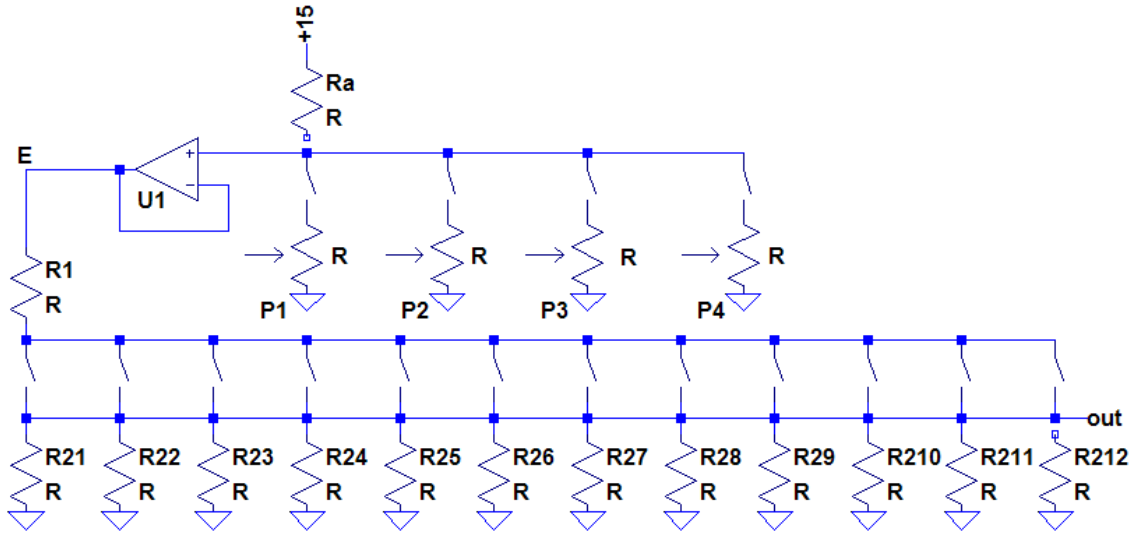
\includegraphics[scale=0.65]{kb-img/keyboard-circuit.png}
	\caption{Circuit du clavier.}
	\label{fig:keyboard-circuit}
\end{figure}

La tension étiquetée \textbf{out} sur la figure
\ref{fig:keyboard-circuit} sera appliquée à l'entrée
du VCO, qui produira ensuite à sa sortie un signal
périodique dont la fréquence est directement 
proportionnelle à l'entrée, selon la convention
\unit{1}{\milli\volt} $=$ \unit{1}{\hertz}. Cette
tension $\text{out}$ est donnée par la formule 
\[ \text{out} = E\frac{R_{2i}}{R_{2i} + R_1} \text{  avec  } i = 1\dots12. \]

Le dimensionnement complet du clavier se base
sur cette formule. En dimensionnant dans un premier
temps le clavier pour l'octave 8, l'obtention
de l'octave 7 est immédiate en divisant la tension
$E$ par deux, et ainsi de suite pour l'octave 6 et 5.
C'est précisément le rôle du réseau de diviseurs
résistifs constitué par les potentiomètres. L'utilisation
de potentiomètres à la place de simples résistances
permet de ``calibrer'' le circuit afin de conserver
une bonne précision (car en pratique l'alimentation
ne vaut pas exactement \unit{15}{\volt}).
% TODO : ajouter la valeur choisie pour les pots.
Arbitrairement, $E$ vaut \unit{14}{\volt} pour l'octave
8 et est divisé par 2 pour chaque octave inférieure.

La présence d'un amplificateur suiveur entre ce premier
réseau de diviseurs résistifs et le suivant est indispensable
pour éviter les ``interférences'' entre résistances.

Le tableau \ref{tab:keyboard-dim} résume le dimensionnement
du clavier. Seules les valeurs standard de la série de Renard
E12 ont été utilisées. En utilisant une combinaison de 3
résistances en séries ou en parallèles, une erreur inférieure
à 0.01\% est garantie (sans tenir compte des tolérances des
résistances). En utilisant une combinaison plus économique
de seulement 2 résistances, des erreurs bien plus grandes
peuvent survenir (de l'ordre de 0.10\% à 0.30\%). Une telle
erreur est encore raisonnable pour l'oreille humaine qui ne
peut pas différencier deux sons dont la fréquence ne diffère
pas de plus de 0.6\%\cite{frequency-jnd}. Cependant, ces erreurs
risquent encore d'être amplifiées dans les blocs suivant du
synthétiseur, il est donc préférable de les minimiser au maximum
dans ce premier bloc.

\begin{table}[ht]
	\centering
		\begin{tabular}{|c|c|}
			\hline
				Résistance & Valeur (en\unit{}{\kilo\ohm}) \\
			\hline
				$R_{1}$ & 10 \\
			\hline
				$R_{21}$ & 82 | (15 + 0.390) \\
			\hline
				$R_{22}$ & 3.3 + (680 | 8.2) \\
			\hline
				$R_{23}$ & 10 + (0.120 | 2.7) \\
			\hline
				$R_{24}$ & 22 | (0.330 + 15) \\
			\hline
				$R_{25}$ & 15 | 1000 | 18 \\
			\hline
				$R_{26}$ & 100 | 220 | 8.2 \\
			\hline
				$R_{27}$ & 150 | (0.150 + 6.8) \\
			\hline
				$R_{28}$ & 8.2 | 39 | 56 \\
			\hline
				$R_{29}$ & 4.7 + (0.820 | 270) \\
			\hline
				$R_{210}$ & 220 | (0.470 + 4.7) \\
			\hline
				$R_{211}$ & 0.56 + (4.7 | 180) \\
			\hline
				$R_{212}$ & 2.7 + (1.8 | 12) \\
			\hline
		\end{tabular}
	\caption{Résumé du dimensionnement du clavier.}
	\label{tab:keyboard-dim}
\end{table}

% TODO : ajouter le calcul de chaque tension out possible
% avec l'erreur relative associé?

\biblio{keyboard}

\end{document}